%%%%%%%%%%%%%%%%%%%%%%%%%%%%%%%%%%%%%%%%%
% Journal Article
% LaTeX Template
% Version 1.4 (15/5/16)
%
% This template has been downloaded from:
% http://www.LaTeXTemplates.com
%
% Original author:
% Frits Wenneker (http://www.howtotex.com) with extensive modifications by
% Vel (vel@LaTeXTemplates.com)
%
% License:
% CC BY-NC-SA 3.0 (http://creativecommons.org/licenses/by-nc-sa/3.0/)
%
% Template modified by Alison Sheltong for STAT 626 Final Project.
%%%%%%%%%%%%%%%%%%%%%%%%%%%%%%%%%%%%%%%%%

%----------------------------------------------------------------------------------------
%	PACKAGES AND OTHER DOCUMENT CONFIGURATIONS
%----------------------------------------------------------------------------------------

\documentclass[twoside,twocolumn]{article}

\usepackage[greek,english]{babel} % Language hyphenation and typographical rules
\usepackage{graphicx}
\usepackage{float, enumitem}
\usepackage{amssymb,amsfonts,textcomp}
\usepackage{caption}
\usepackage{lmodern}
\usepackage{booktabs} % Horizontal rules in tables

\usepackage{hyperref} % For hyperlinks in the PDF

\usepackage{blindtext} % Package to generate dummy text throughout this template - helpful for double checking spaccing.

\usepackage[utf8x]{inputenc} %Because I like this one better than the one in the template
\usepackage{natbib}
\bibliographystyle{apalike}


\usepackage[margin=.75 in, hmarginratio=1:1,top=32mm,columnsep=20pt]{geometry} % Document margins, provided extra space for us with smaller margins than the default.

\usepackage{enumitem} % Customized lists
\setlist[itemize]{noitemsep} % Make itemize lists more compact

\usepackage{abstract} % Allows abstract customization - The italics for example.
\renewcommand{\abstractnamefont}{\normalfont\bfseries} % Set the "Abstract" text to bold
\renewcommand{\abstracttextfont}{\normalfont\small\itshape} % Set the abstract itself to small italic text

\usepackage{fancyhdr} % Headers and footers
\pagestyle{fancy} % All pages have headers and footers
\lhead{\bfseries Group 4}
\chead{\bfseries STAT 626: Time Series Analysis}
\rhead{\bfseries US Unemployment Trends} 
\lfoot{}
\cfoot{\thepage}
\rfoot{} 


\usepackage{titling} % Customizing the title section 

%----------------------------------------------------------------------------------------
%	TITLE SECTION
%----------------------------------------------------------------------------------------
\setlength{\droptitle}{-4\baselineskip} % Move the title up

\pretitle{\begin{center}\huge\bfseries} % Article title formatting
\posttitle{\end{center}} % Article title closing formatting
\title{US Unemployment Trends} % Article title
\author{%
\textsc{Joseph Blubaugh}\thanks{Plots, Data Prep, Code Management} \\[1ex] % Your name
\normalsize Statistics\\ % Your institution
%\normalsize \href{mailto:john@smith.com}{john@smith.com} % Your email address
\and % Uncomment if 2 authors are required, duplicate these 4 lines if more
\textsc{Sean Roberson}\thanks{Presentor} \\[1ex] % Second author's name
\normalsize Mathematics, Industrial\\ % Second author's institution
\and 
\textsc{Akarshan Puri}\thanks{Model selection and fitting} \\[1ex] 
\normalsize Electrical Engineering\\ 
\and 
\textsc{Alison Shelton}\thanks{Write-up} \\[1ex] 
\normalsize Statistics\\ 
\and 
\textsc{Travis Lilley}\thanks{Diagnostics} \\[1ex] 
\normalsize Statistics\\ 
\and
\textsc{Bo Pang}\thanks{Model fitting and plots} \\[1 ex]
\normalsize Psychology, Statistics
\vspace*{.5 cm}
}
%\institute[Texas A\&M] % I'm not sure yet how to add this in with the way that I put in the author names.
	%	{Texas A\&M \newline College Station, Texas}
\date{July 25, 2016 \vspace*{.25 cm}} % Final write-up due date plus a bit of extra space
\renewcommand{\maketitlehookd}{%
\begin{abstract}
\noindent The information from above is from the original presentation.  The links as to who did what should be modified probably at the end.  This is just a starting point. Also the abstract should be written last so I thought it was a good place to put this information.

\vspace*{.25 cm}
\noindent The writeup below has dummy text so I could set up the sections. I also moved some of the older write-up text to this document to start it all up.
\end{abstract}
}



%----------------------------------------------------------------------------------------

\begin{document}
%----------------------------------------------------------------------------------------
%	Appendices: These are temporary
%----------------------------------------------------------------------------------------

\section{Appendices}
\appendix

\section{Research to Include Later}

``The estimation of unobserved components: trend-cycle, seasonal and irregular component was made with SEATS program based on ARIMA models. Seasonally adjusted series were obtained by removing the seasonal component from the original data. Trend was obtained by removing the irregular component from the seasonally adjusted series'' \citep{VOINEAGU2012}.

``A possible leading indicator variable for the unemployment rate is the number of initial claims of unemployment'' \citep{Montgomery1998}.

\section{commentary moved to the end}

\begin{figure}[htb]
    	\centering
     	\caption{Forcasting with ARIMA and VAR models}
     	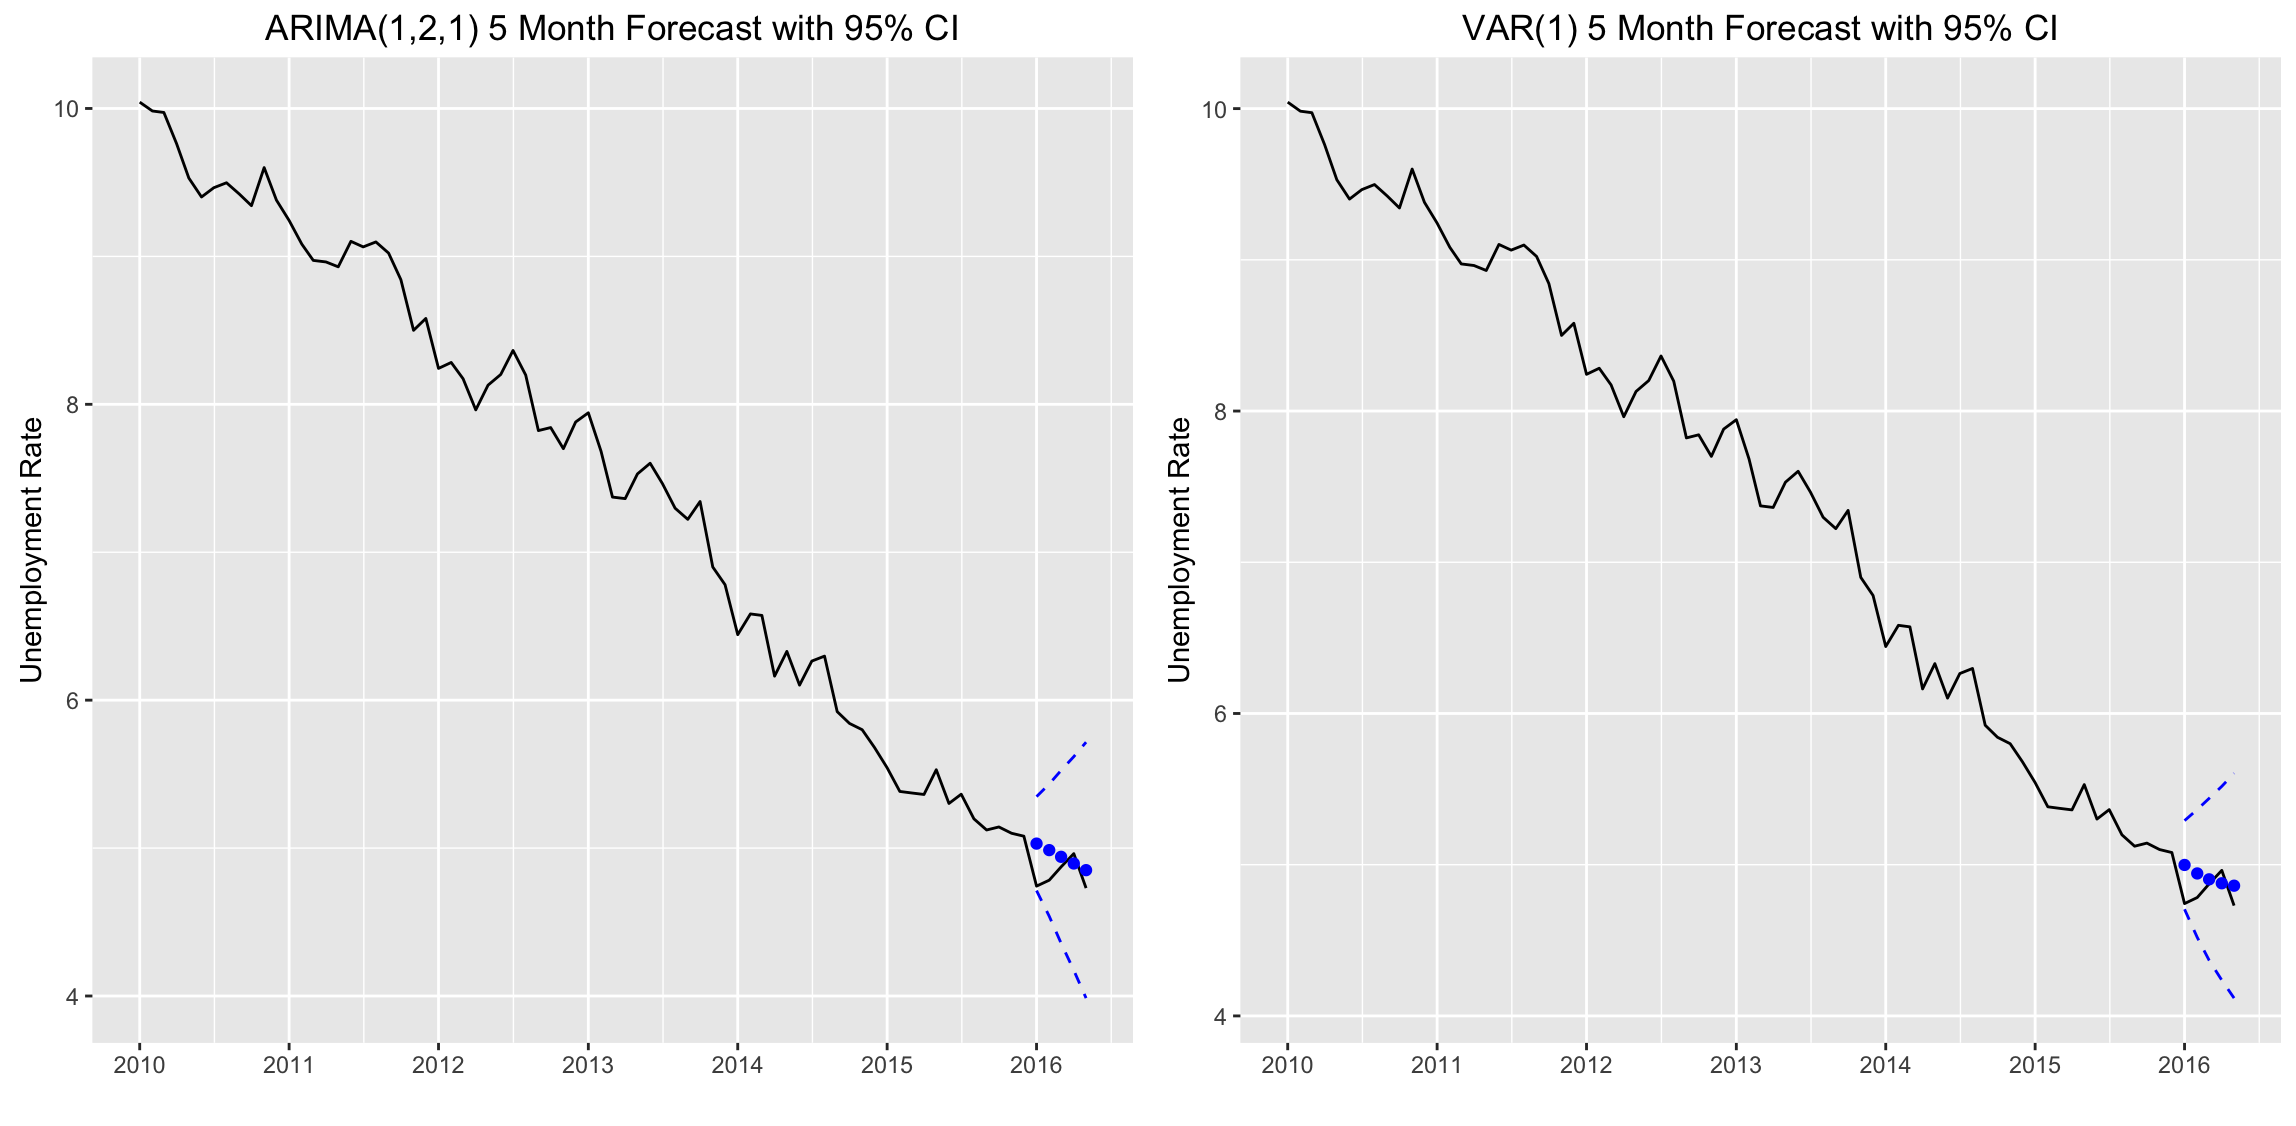
\includegraphics[width=\linewidth]{images/forcasts}
     	\label{fig:forcasts}
      \end{figure}
      
       \begin{figure}[htb]
    	\centering
     	\caption{3 year forcasts}
     	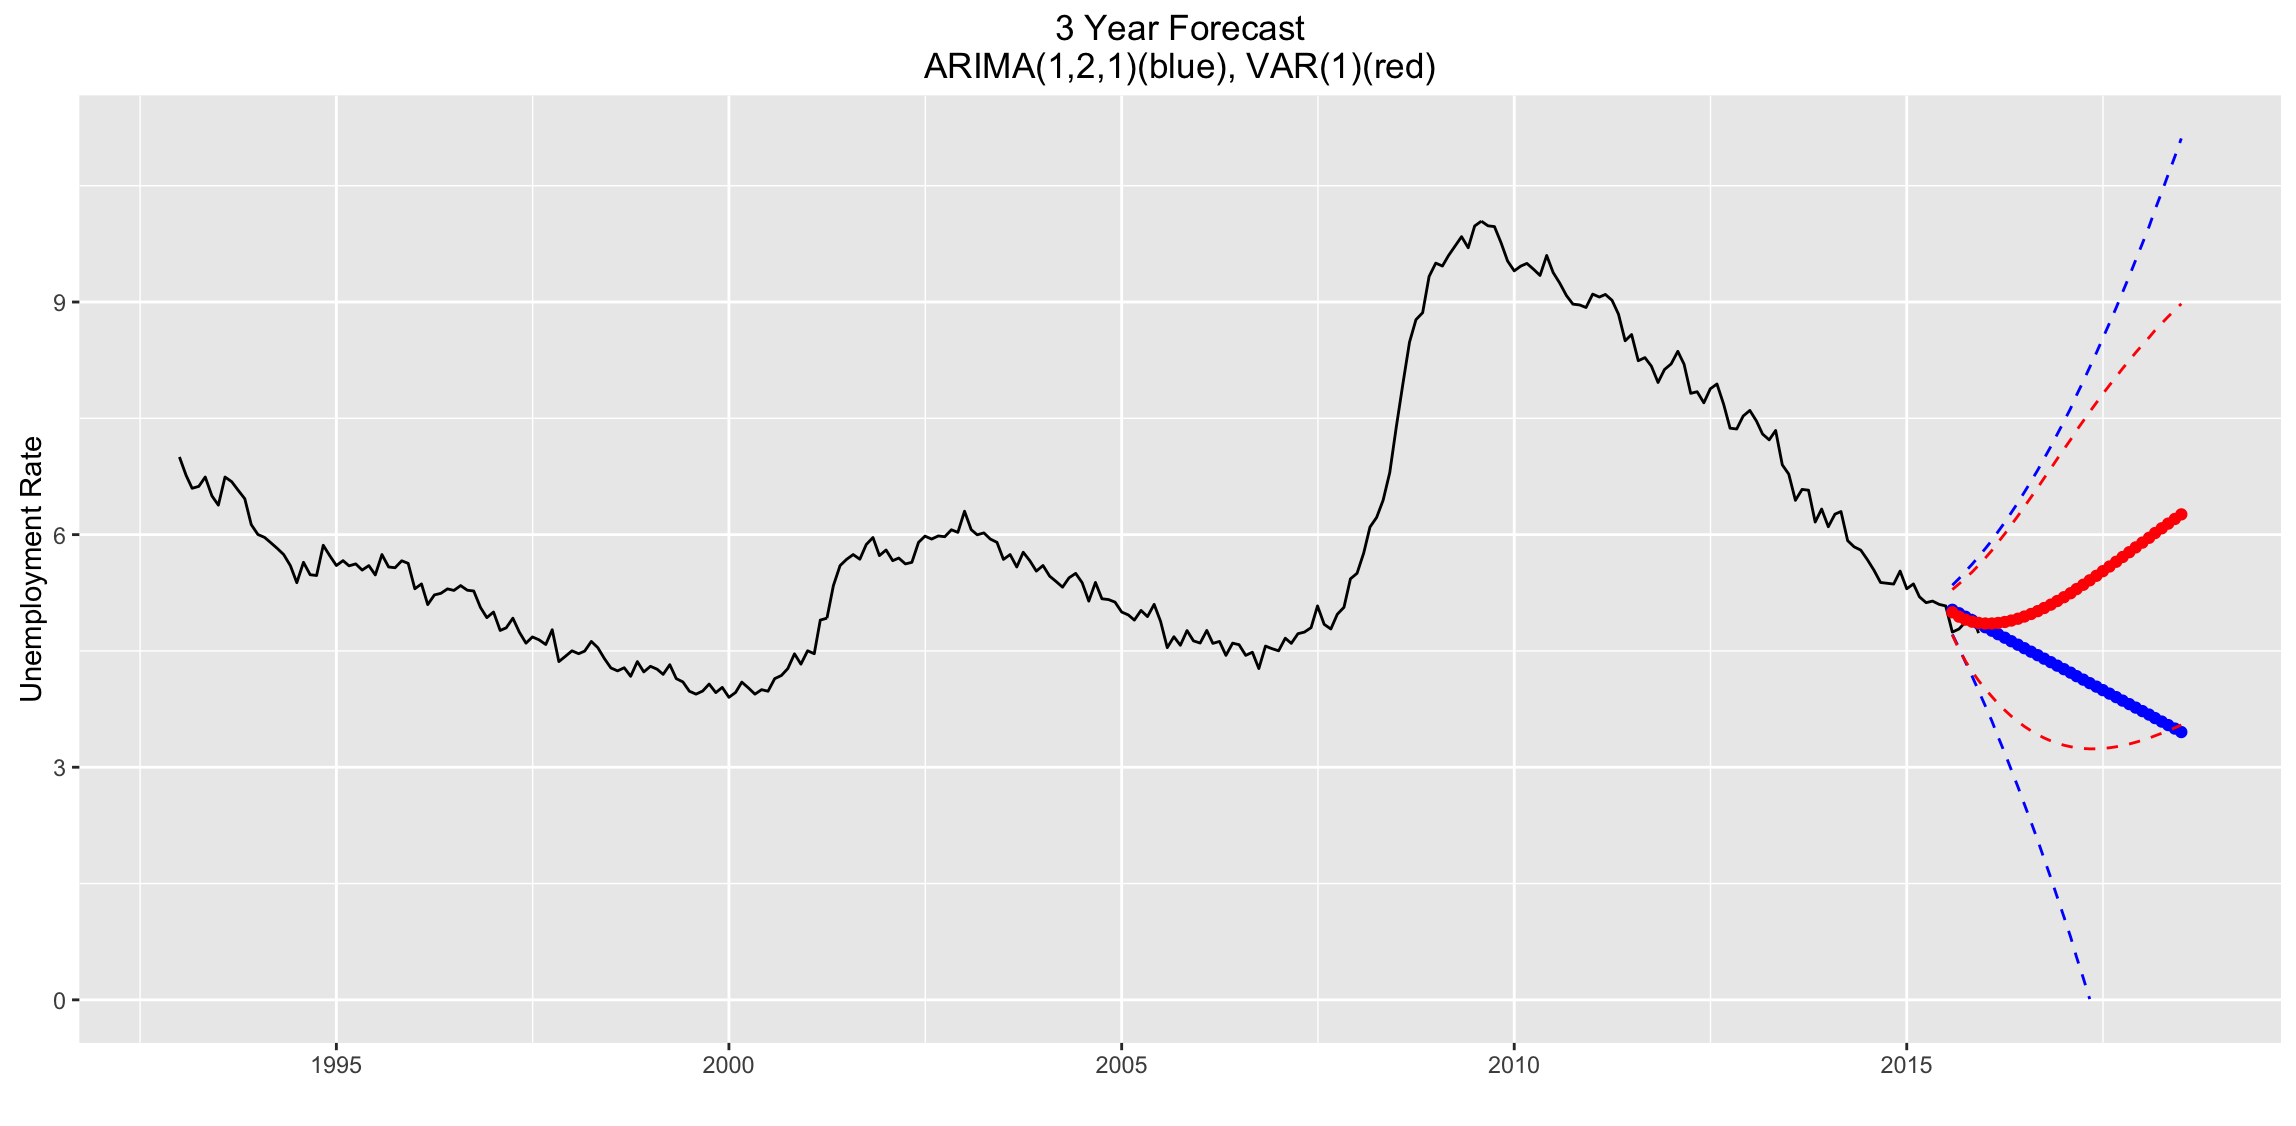
\includegraphics[width=\linewidth]{images/forcast3}
     	\label{fig:forcasts2}
      \end{figure}
      
      The ARIMA(1, 2, 1) predicts that unemployment will continue to decrease indefinitely, which we know can't be true. The VAR(1) model shows a much more accurate picture in the long run.

      
      I am glad to start doing some forecasting. I did some with the ARIMA(1, 2, 1) seasonally adjusted, no predictors. It's in the RScript "forecasting."

What other potential models are we considering? My only concern is that if we choose a model with predictors, we will have to forecast those predictors before we forecast the unemployment rate.

In case we go with the ARIMA(1, 2, 1) model for the seasonally adjusted data with no predictors, here are some forecast plots. I uploaded them in the Plots folder, too.

The graphs are for the h = 5, 12, and 24 step ahead forecasts. The first three were generated by sarima( ), and the last three by Arima( ). Personally, I think the last three look better. I think it's good to have a picture of the forecast in the context of all the data. I will play around with sarima( ) to see if I can adjust the default axes to accommodate all past data.


 \begin{figure}[H]
    	\centering
     	\caption{Plots described above}
     	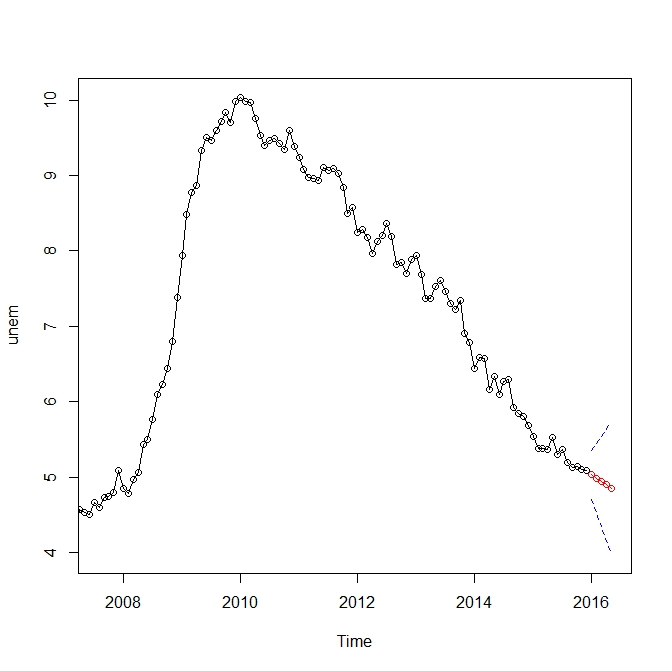
\includegraphics[width=.9\linewidth]{images/fore1}
 \end{figure}
 
  \begin{figure}[H]
    	\centering
     	\caption{Plots described above}
     	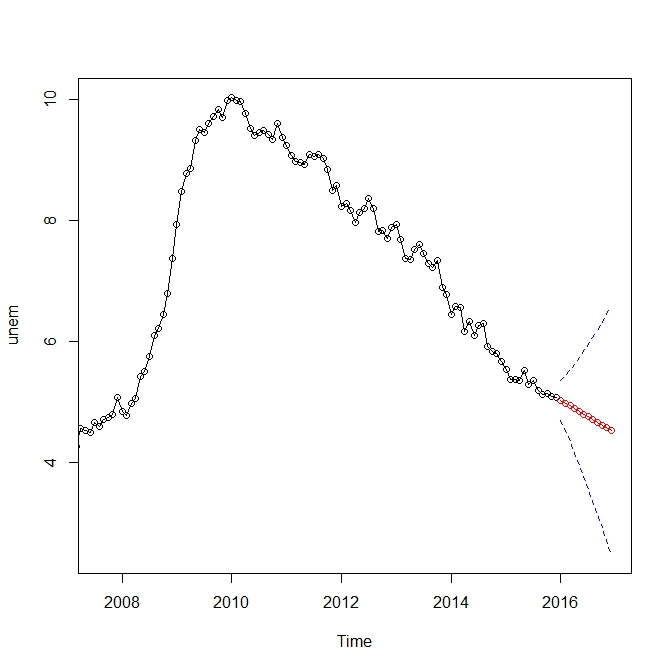
\includegraphics[width=.9\linewidth]{images/fore2}
     	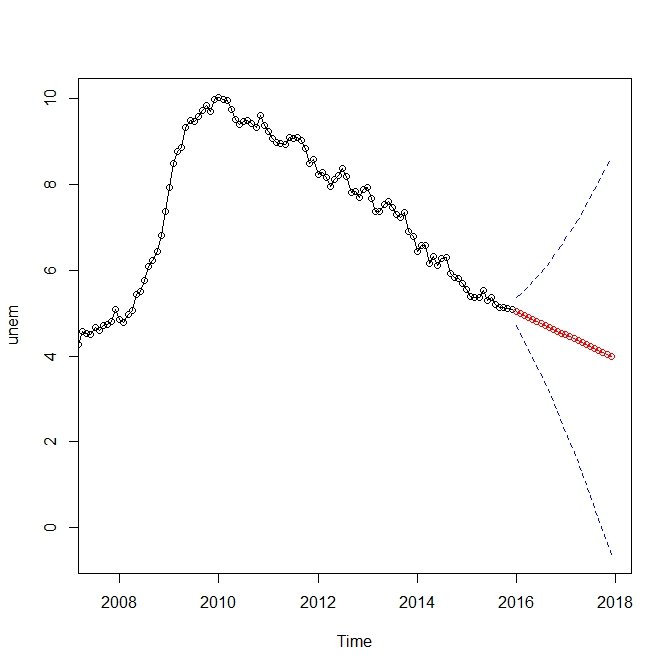
\includegraphics[width=.9\linewidth]{images/fore3}
     	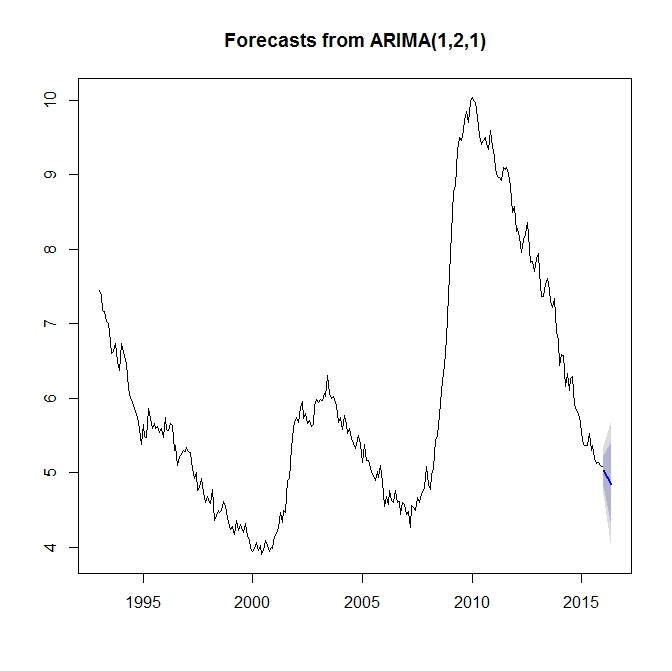
\includegraphics[width=.9\linewidth]{images/fore4}
 \end{figure}

  \begin{figure}[H]
    	\centering
     	\caption{Plots described above}
     	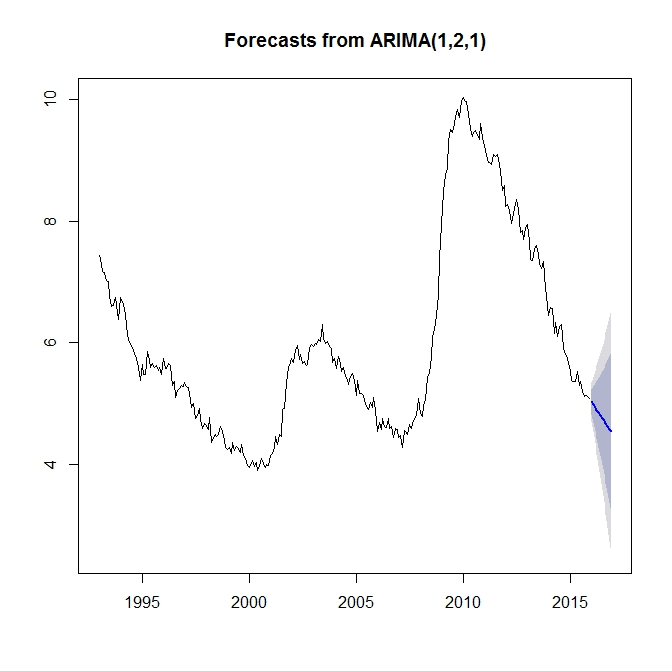
\includegraphics[width=.8\linewidth]{images/fore5}
     	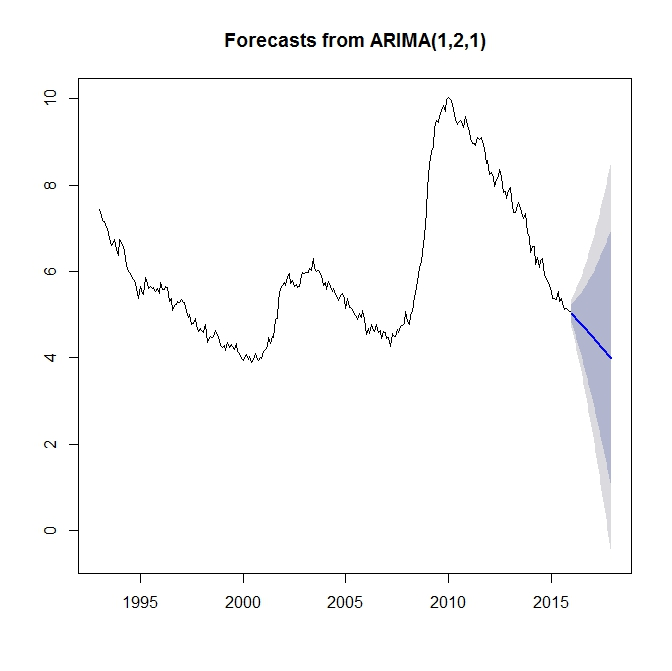
\includegraphics[width=.7\linewidth]{images/fore6}
     	\caption{Plot described below}
     	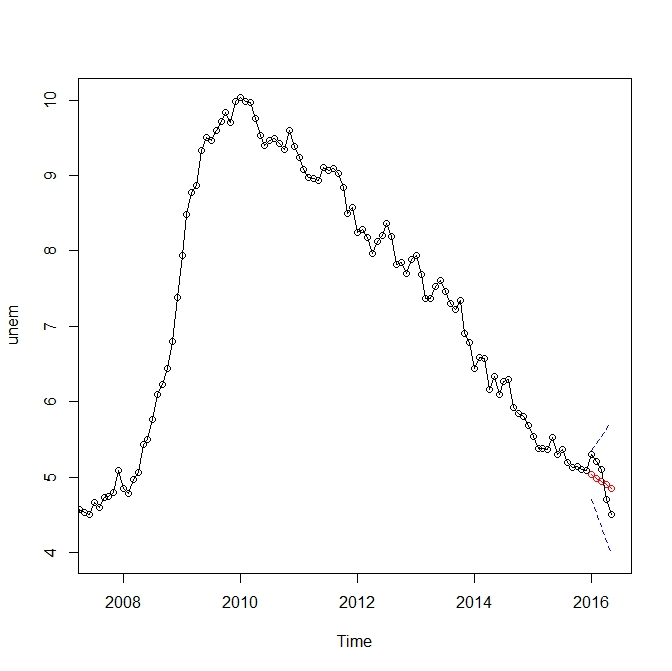
\includegraphics[width=.7\linewidth]{images/fore7}
 \end{figure}
 
 And here is a plot of the first five forecasted values (red) along with the actual observed values (black) from 2016. 
 
 I looked at the FRED website where we got our data, and it looks like the unemployment for June 2016 has been posted at 5.1\%. We could compare that to our predictor for June 2016 as well.

Here is a plot from Arima( ) that shows the predicted values through June 2016 (blue) and the observed values (black).

I put all the code for my plots in the RSCript folder and named it ``forecasting plots.''


Of the models we have discussed so far, I think the ARIMA(1, 2, 1) is best. It had the best diagnostics and the lowest AIC.

I added some predictors to the ARIMA(1, 2, 1), and only retail seemed significant. However, its coefficient is so small that I argue we don't need it.

I then did some forecasting for the ARIMA(1, 2, 1) as well as two ARIMA(1, 2, 1) models with predictors. I then compared our predicted values for 2016 unemployment with the actual values:

\begin{verbatim}
Jan 2016: actual 5.3 , predicted = 5.0
Feb 2016: actual 5.2 , predicted = 5.0

Mar 2016: actual 5.1 , predicted = 4.9
Apr 2016: actual 4.7 , predicted = 4.9
May 2016: actual 4.5 , predicted = 4.9

Overall, I think the ARIMA(1, 2, 1) is very good.

I uploaded all of my code as "forecasting 7_21_16".

\end{verbatim}

  \begin{figure}[htb]
    	\centering
     	\caption{with June 2016}
     	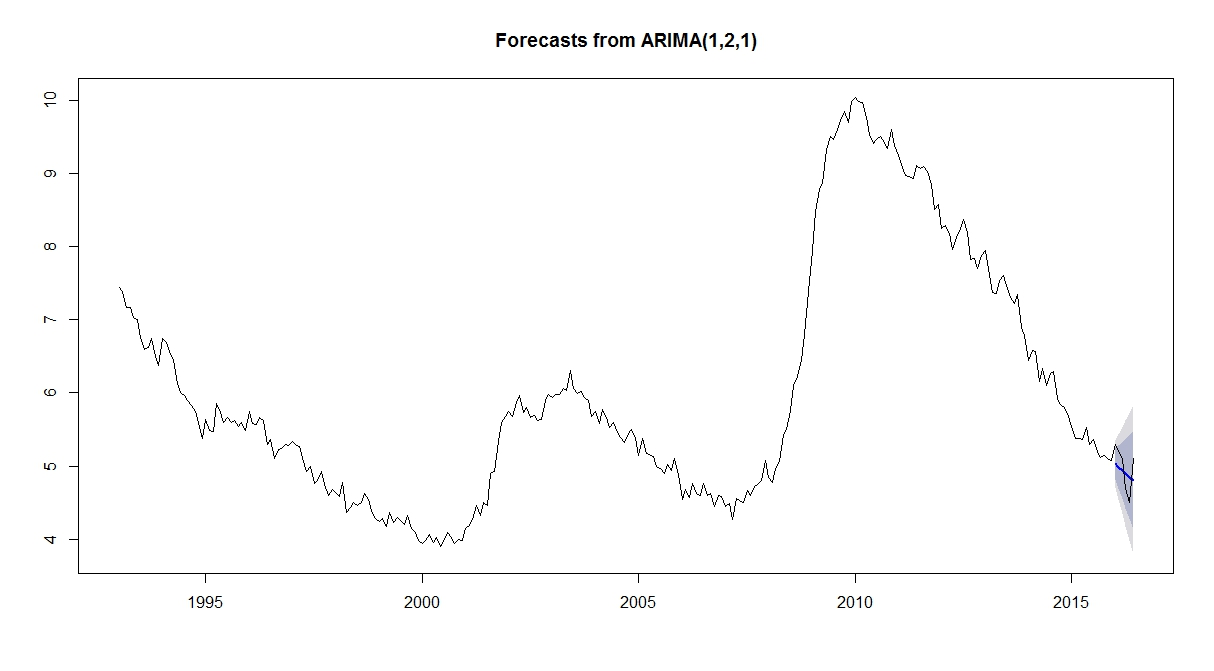
\includegraphics[width=\linewidth]{images/forejune}
 \end{figure}
 
The professor seems to like the idea of splitting the data into training and validation sets. We didn't split the data but luckily we have the new 5 months data as a validation set. From looking at the plots, it seems hard to distinguish the performance of two models. I computed the mean squared error of forecasting of the two best models. 0.01505823 for ARIMA(1,2,1) and 0.009663836 for VAR(1). This quantitative measure also supports this VAR(1) model. Hope this would help a bit when we are comparing the two models.  
  \begin{figure}[htb]
    	\centering
     	\caption{with June 2016}
     	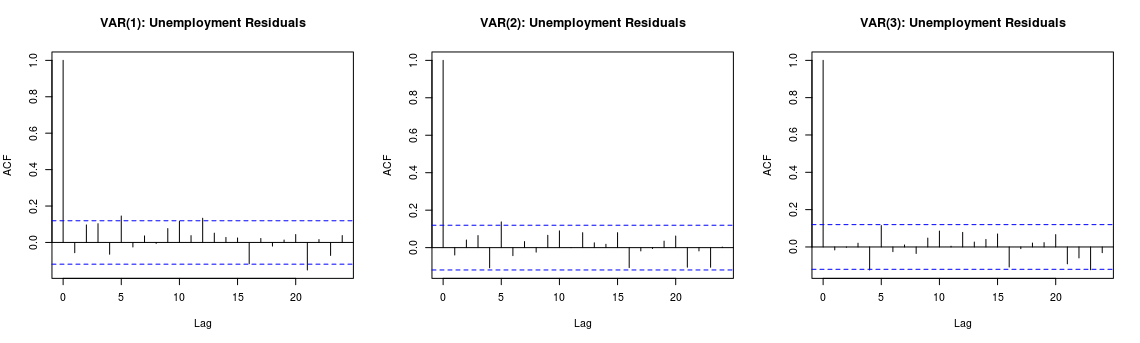
\includegraphics[width=\linewidth]{images/varUnemresid}
 \end{figure}
 
 Here is a plot of the unemployment series in the best performing model by AIC: Var(2) with lagged xregs.
 
   \begin{figure}[htb]
    	\centering
     	\caption{fit and residuals}
     	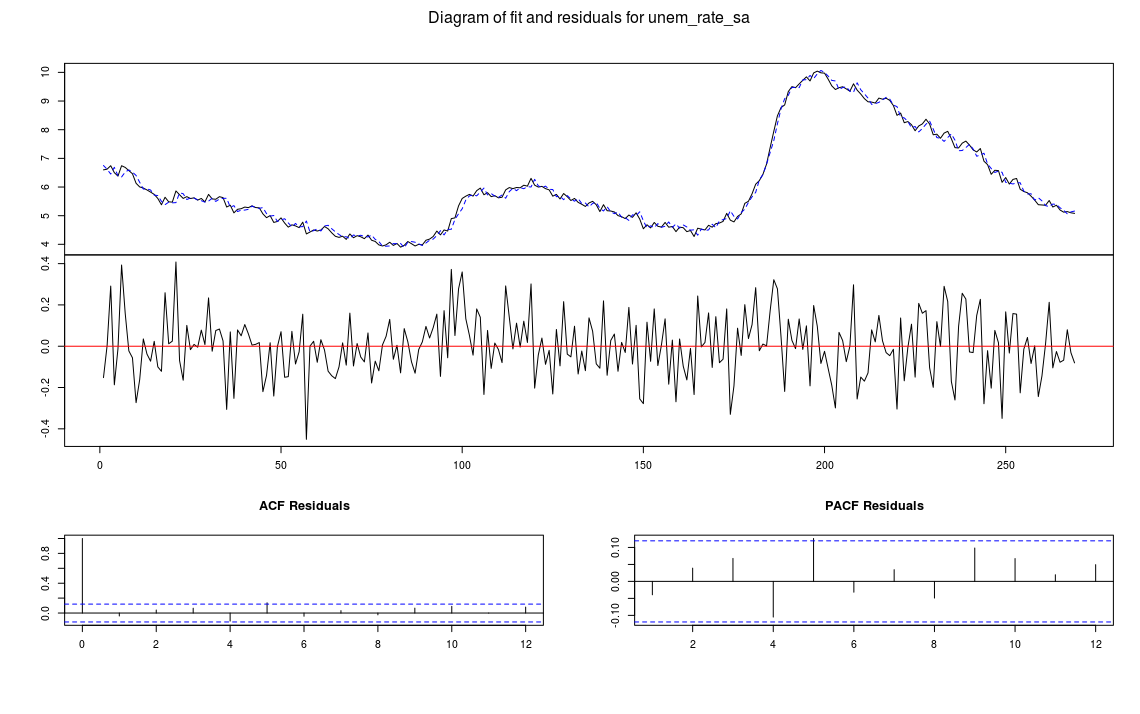
\includegraphics[width=\linewidth]{images/unem_rate_fit_resid}
 \end{figure}
 
 There is also forecasting functionality in the package which is nice because in the case of an ARIMA model with xregs, you dont have to forecast the xregs. Vars will do that for you since all of they are essentially AR(p) models that only use lagged values to forecast.
 
    \begin{figure}[htb]
    	\centering
     	\caption{Var(2) Forcast 5 mo}
     	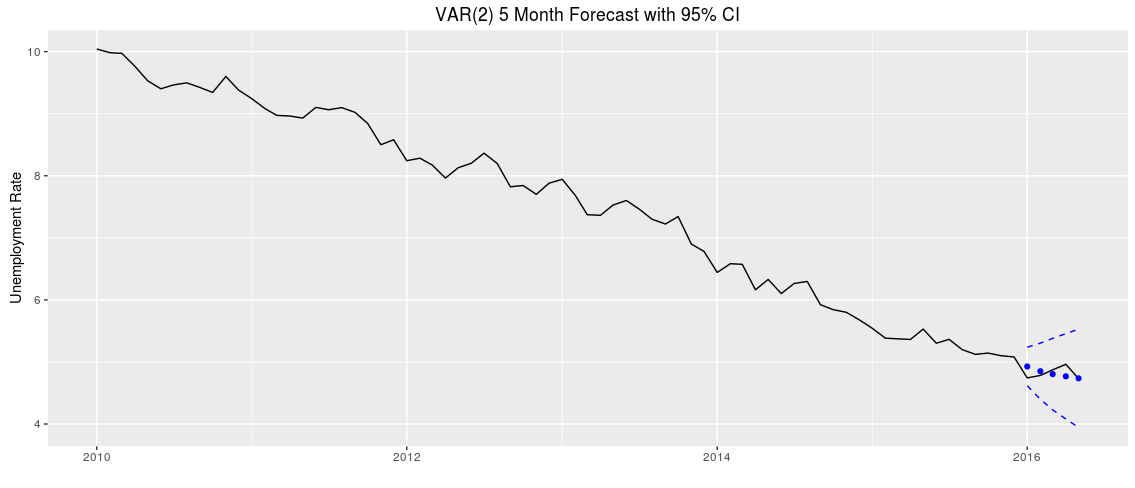
\includegraphics[width=\linewidth]{images/var25mo}
 \end{figure}
 
I also built a few VAR models. By VARselect, BIC suggests VAR(1) HQ suggest VAR(2). The VAR(1) results only show the \begin{verbatim}retail_sales_sa.l1 and recession_ind.l1\end{verbatim} besides \begin{verbatim}unem_rate_sa.l1\end{verbatim} were significant predictors. I checked the correlation among these predictors and found that variables \begin{verbatim}industrial_production, manufacturers_new_orders, \end{verbatim} \begin{verbatim}house_price_sa, construction_spend, and retail_sales\end{verbatim} are highly correlated.

    \begin{figure}[htb]
    	\centering
     	\caption{Scatterplot matrix}
     	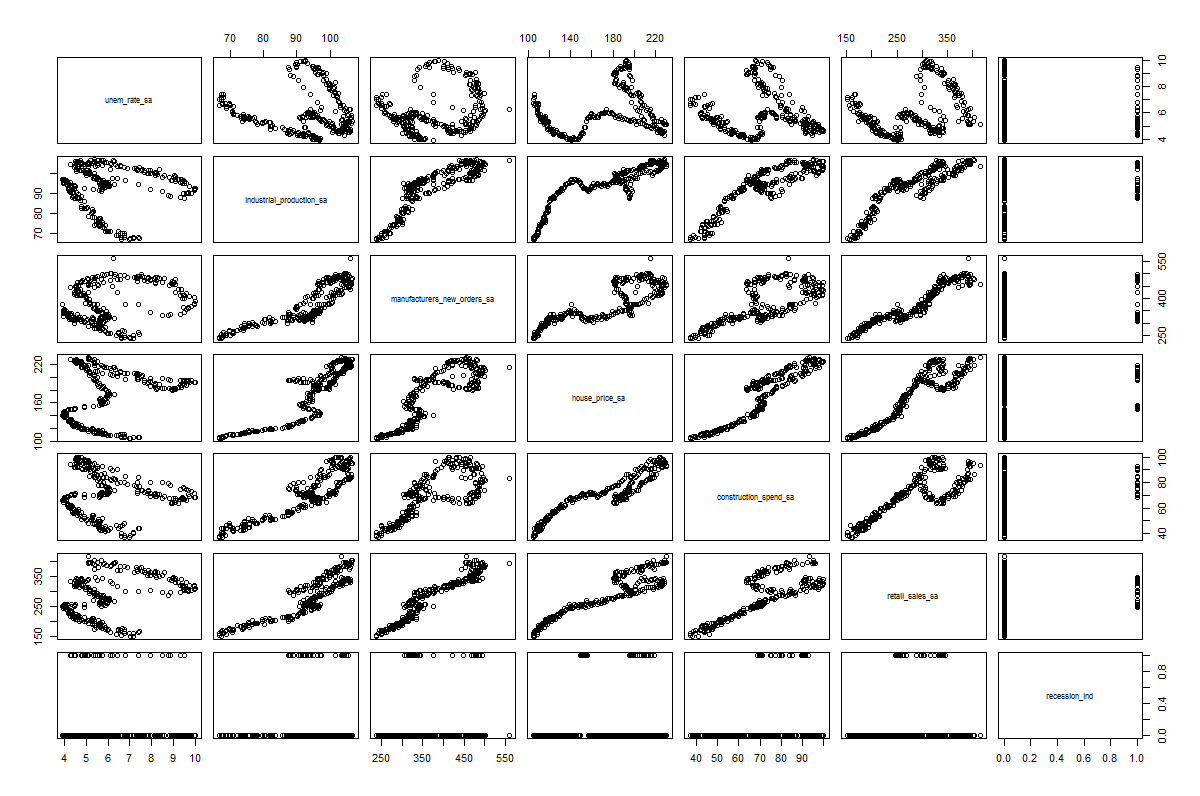
\includegraphics[width=\linewidth]{images/varcorrelation}
 \end{figure}

It might be reasonable to leave out some highly correlated variables. Thus, I then fitted two models with only \begin{verbatim}unem_rate, retail_sales, and recession_ind\end{verbatim}. Here are the AICs and BICs.

\begin{verbatim}
AIC(M1$varresult$unem_rate_sa) # -253.317
AIC(M2$varresult$unem_rate_sa) # -252.6457
AIC(M3$varresult$unem_rate_sa) # -247.1147
AIC(M4$varresult$unem_rate_sa) # -251.6351

BIC(M1$varresult$unem_rate_sa) # -217.1493
BIC(M2$varresult$unem_rate_sa) # -191.2225
BIC(M3$varresult$unem_rate_sa) # -225.414
BIC(M4$varresult$unem_rate_sa) # -219.117

AICs suggest the original VAR(1) model. 
The BICs suggest the VAR(1) with only three variables. 
\end{verbatim}

    \begin{figure}[htb]
    	\centering
     	\caption{Plots of above}
     	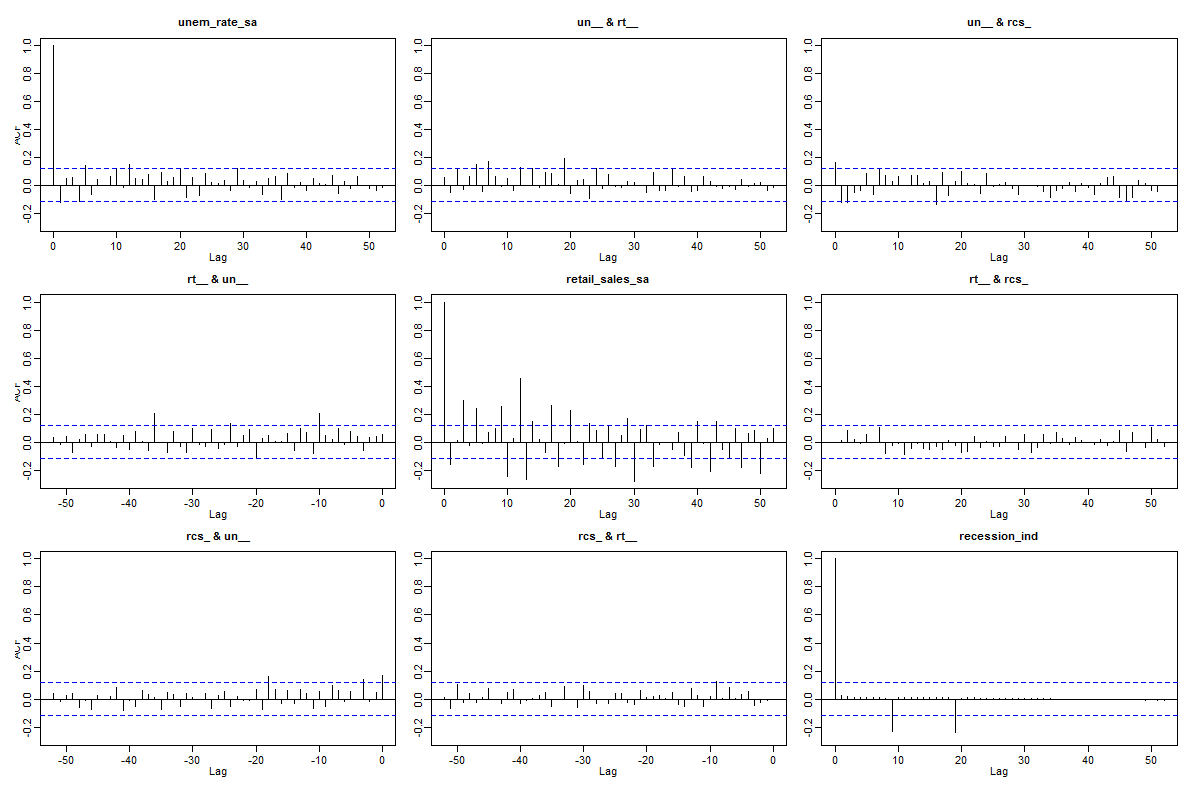
\includegraphics[width=\linewidth]{images/boplots}
 \end{figure}


\textit{These tables are included earlier.}

5 Month Forecasts for the 2 best Models

Since we decomposed and adjusted the seasonal data ourselves, it differs slightly from what you would see on the BLS website so I applied the same seasonal adjustment to the first 5 months of unemployment that came with the original data set. Overall the two plots are very similar.

It also looks like the VAR model produced a slightly better forecast over this period, however the confidence intervals of the models overlap substantially.

The forecasts start to look significantly different when you look at the longer term forecasts. This plot shows a 36 month forecast for the two best models. We can see how the confidence interval of the ARIMA model quickly explodes, perhaps indicating that it is not a good choice for long term forecasts.

\textit{All of the previously mentioned plots are already included earlier except for:}
    \begin{figure}[htb]
    	\centering
     	\caption{Other plot}
     	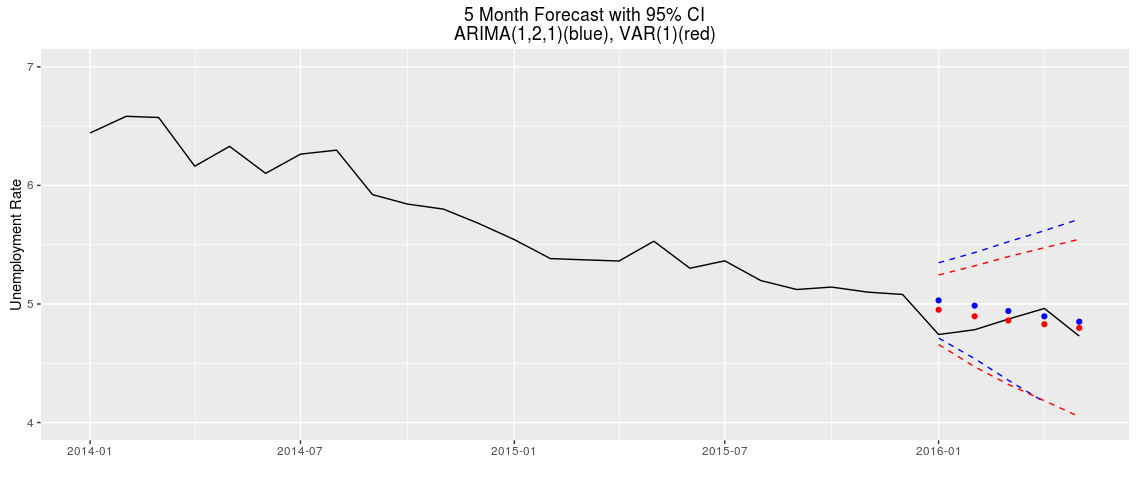
\includegraphics[width=\linewidth]{images/arimavarforcastalso}
 \end{figure}
 


Updated the VAR to not include the insignificant variables I mentioned. The plots in \(All_Final_Models.r\) will reflect this... here are the updated tables now that those variables have been dropped. This matches the VAR equation i posted yesterday.


The professor seems to like the idea of splitting the data into training and validation sets. We didn't split the data but luckily we have the new 5 months data as a validation set. From looking at the plots, it seems hard to distinguish the performance of two models. I computed the mean squared error of forecasting of the two best models. 0.01505823 for ARIMA(1,2,1) and 0.009663836 for VAR(1). This quantitative measure also supports this VAR(1) model. Hope this would help a bit when we are comparing the two models. 

% latex table generated in R 3.2.4 by xtable 1.8-2 package
% Mon Jul 25 11:23:13 2016
\begin{table}[ht]
\centering
\begin{tabular}{rrrrrrrrr}
  \hline
 & unemployment & arima.pred & arima.pred.lwr & arima.pred.upr & var.pred & var.pred.lwr & var.pred.upr & dt \\ 
  \hline
73 & 4.74 &  &  &  & 5.00 & 4.71 & 5.29 & Jan \\ 
  74 & 4.78 &  &  &  & 4.94 & 4.52 & 5.36 & Feb \\ 
  75 & 4.87 &  &  &  & 4.90 & 4.37 & 5.44 & Mar \\ 
  76 & 4.96 &  &  &  & 4.88 & 4.24 & 5.52 & April \\ 
  77 & 4.73 &  &  &  & 4.86 & 4.12 & 5.60 & May \\ 
   \hline
\end{tabular}
\end{table}

% latex table generated in R 3.2.4 by xtable 1.8-2 package
% Mon Jul 25 11:27:03 2016
\begin{table}[ht]
\centering
\begin{tabular}{rrrrrrrrr}
  \hline
 & unemployment & arima.pred & arima.pred.lwr & arima.pred.upr & var.pred & var.pred.lwr & var.pred.upr & dt \\ 
  \hline
73 & 4.74 & 5.03 & 4.71 & 5.35 & 5.00 & 4.71 & 5.29 & Jan-16 \\ 
  74 & 4.78 & 4.99 & 4.54 & 5.43 & 4.94 & 4.52 & 5.36 & Feb-16 \\ 
  75 & 4.87 & 4.94 & 4.36 & 5.53 & 4.90 & 4.37 & 5.44 & Mar-16 \\ 
  76 & 4.96 & 4.90 & 4.17 & 5.62 & 4.88 & 4.24 & 5.52 & Apr-16 \\ 
  77 & 4.73 & 4.85 & 3.99 & 5.72 & 4.86 & 4.12 & 5.60 & May-16 \\ 
   \hline
\end{tabular}
\end{table}

% latex table generated in R 3.2.4 by xtable 1.8-2 package
% Mon Jul 25 11:27:03 2016
\begin{table}[ht]
\centering
\caption{2016 Predicted Values}
\begin{tabular}{rrrrrrrrr}
  \hline
 & unemployment & arima.pred & arima.pred.lwr & arima.pred.upr & var.pred & var.pred.lwr & var.pred.upr & dt \\ 
  \hline
73 & 4.74 & 5.03 & 4.71 & 5.35 & 5.00 & 4.71 & 5.29 & Jan-16 \\ 
  74 & 4.78 & 4.99 & 4.54 & 5.43 & 4.94 & 4.52 & 5.36 & Feb-16 \\ 
  75 & 4.87 & 4.94 & 4.36 & 5.53 & 4.90 & 4.37 & 5.44 & Mar-16 \\ 
  76 & 4.96 & 4.90 & 4.17 & 5.62 & 4.88 & 4.24 & 5.52 & Apr-16 \\ 
  77 & 4.73 & 4.85 & 3.99 & 5.72 & 4.86 & 4.12 & 5.60 & May-16 \\ 
   \hline
\end{tabular}
\end{table}


% latex table generated in R 3.2.4 by xtable 1.8-2 package
% Mon Jul 25 11:36:43 2016
\begin{table}[ht]
\centering
\caption{2016 Predictions from Multivariate ARIMA(1,2,1)}
\begin{tabular}{rrrrrrr}
  \hline
 Date & Actual Unemployment & Prediction & Lower CI & Upper CI & Residual \\ 
  \hline
Jan-16 & 4.74 & 5.03 & 4.71 & 5.35 & -0.29 \\ 
Feb-16 & 4.78 & 4.99 & 4.54 & 5.43 & -0.20 \\ 
Mar-16 & 4.87 & 4.94 & 4.36 & 5.53 & -0.07 \\ 
Apr-16 & 4.96 & 4.90 & 4.17 & 5.62 & 0.07 \\ 
May-16 & 4.73 & 4.85 & 3.99 & 5.72 & -0.12 \\  \hline
   \hline
\end{tabular}
\end{table}

\end{document}